% Gemini theme
% https://github.com/anishathalye/gemini

\documentclass[final,20pt]{beamer}

% ====================
% Packages
% ====================

\usepackage[ngerman]{babel}
\usepackage[T1]{fontenc}
\usepackage{lmodern}
\usepackage[size=a1,orientation=portrait,scale=1.2]{beamerposter}
\usetheme{gemini}
\usecolortheme{gemini}
\usepackage{graphicx}
\usepackage{tikz}
\usepackage{pgfplots}
\usepackage{svg}

% ====================
% Lengths
% ====================

% If you have N columns, choose \sepwidth and \colwidth such that
% (N+1)*\sepwidth + N*\colwidth = \paperwidth
\newlength{\sepwidth}
\newlength{\colwidth}
\setlength{\sepwidth}{0.02\paperwidth}
\setlength{\colwidth}{0.47\paperwidth}

\newcommand{\separatorcolumn}{\begin{column}{\sepwidth}\end{column}}
\addto\extrasngerman{\def\figureautorefname{Abb.}}
% ====================
% Title
% ====================

\title{Apoplexy - Ein Fitnesstracker zur Rehabilitation von Schlaganfall-Patienten?}

\author{Lukas Rost}
\institute{Albert-Schweitzer-Gymnasium Erfurt}

% ====================
% Body
% ====================

\begin{document}

\begin{frame}[t]
\begin{columns}[t]
\separatorcolumn

\begin{column}{\colwidth}
   \begin{alertblock}{Aufbau und Schaltung des Geräts}
  	\begin{itemize}
  		\item \textbf{Elektromyografie-Sensor:}
  		\begin{itemize}
  			\item Messung der Stärke der Armmuskel-Kontraktionen
  			\item Messung anhand von Potentialänderungen auf der Haut
  			\item drei Oberflächenelektroden
  			\item Verstärkung und Filterung
  			\item Ausgabe eines Analogsignals (Spannung) proportional zur Muskelaktivität
  		\end{itemize}
  		\item \textbf{Mikrocontroller Atmel ATmega:}
  		\begin{itemize}
  			\item Weitergabe der Sensordaten an den Bluetooth-Chip
  			\item 8-Bit-Mikrocontroller mit RISC-Architektur (reduzierter Befehlssatz, aber schneller)
  			\item Harvard-Struktur mit getrennten Speicherbereichen für Befehle und Daten
  			\item Schnittstellen: u.a. UART und Analog-Digital-Wandler
  			\item diese können über Portadressen angesprochen werden
  			\item gut für den Einsatzzweck geeignet (schnell, besitzt alle nötigen Schnittstellen)
  		\end{itemize}
  		\item \textbf{Bluetooth-Chip HC-05:}
  		\begin{itemize}
  			\item drahtlose Kommunikation mit dem Android-Mobilgerät über Funk 
  			\item arbeitet nach dem Bluetooth-Standard
  			\item alle nötigen Bestandteile auf einem Chip integriert
  			\item Kommunikation zwischen Mikrocontroller und HC-05 per UART-Schnittstelle (digitale serielle Schnittstelle zur Datenübertragung)
  		\end{itemize}
  		\item \textbf{Quarzoszillator und Kondensatoren:}
  		\begin{itemize}
  			\item eingebauter Schwingquarz mit fester Frequenz
  			\item liefert genauen Systemtakt für störungsfreie UART-Kommunikation
  			\item muss über die Einstellungen (Fuses) des Mikrocontrollers angewählt werden
  			\item Kondensatoren für ordnungsgemäße Funktion notwendig
  		\end{itemize}
  		\item \textbf{Batterie} zur Stromversorgung der Schaltung
  	\end{itemize}
  
  	\begin{figure}[H]
  		\centering
  		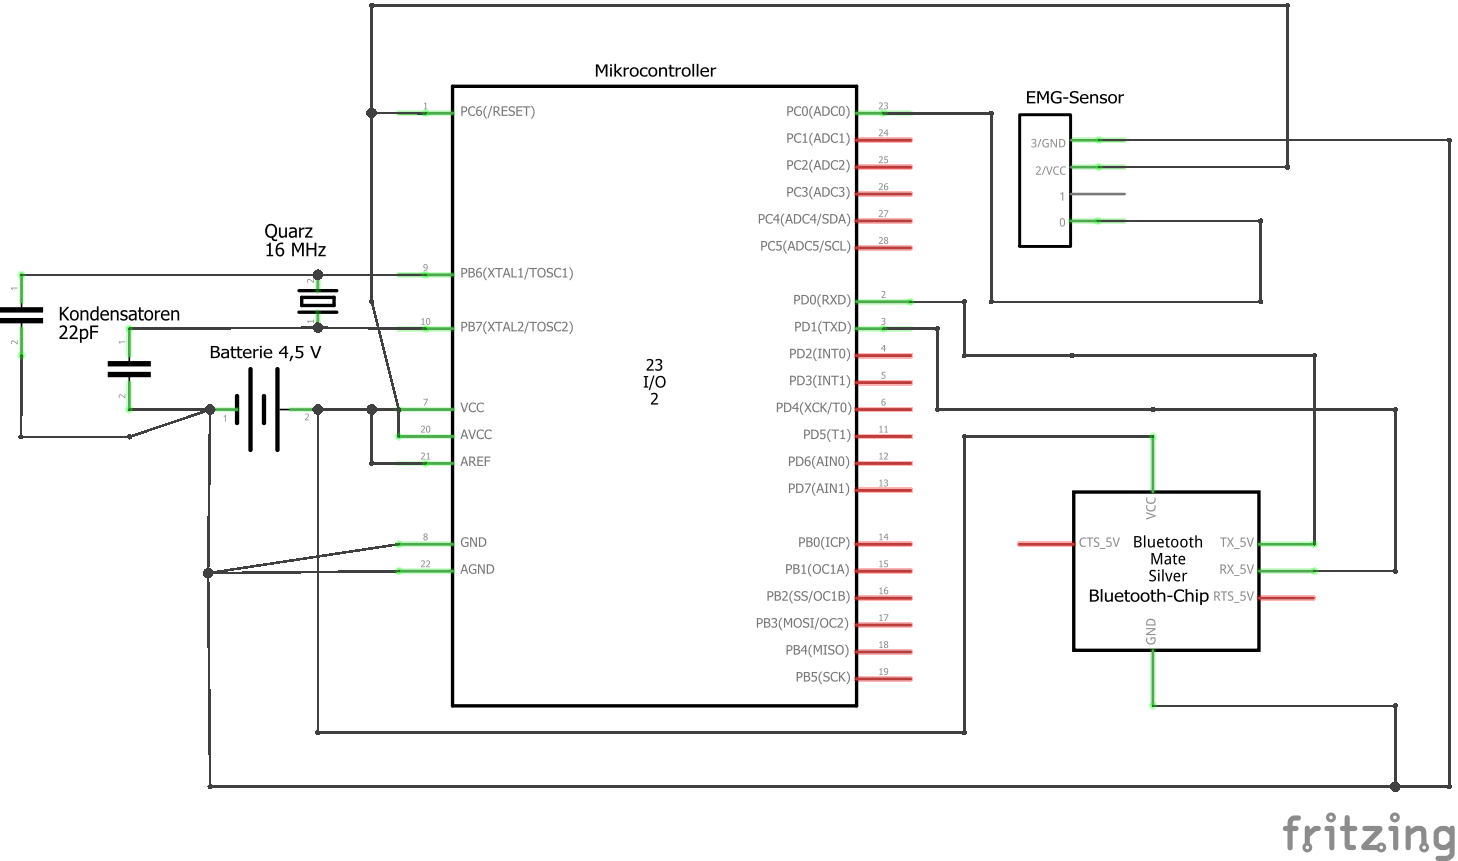
\includegraphics[width=0.8\colwidth]{pics/mikrocontroller-schaltplan}
  		\caption{vereinfachter Schaltplan}
  		\label{fig:mcsp}
  	\end{figure}
  \end{alertblock}

  \begin{alertblock}{Programmierung des Geräts}
  	\begin{itemize}
  		\item Programm wird auf dem Mikrocontroller ausgeführt
  		\item wurde in der Programmiersprache C programmiert
  		\item Nutzung der AVR-Bibliotheken von Atmel
  		\item nach dem Start: Initialisierung der Schnittstellen und Funktionen
  		\item Senden der aktuell gemessenen Spannung über UART im Abstand einer halben Sekunde
  		\item Messung per Analog-Digital-Wandler
  		\item Schnittstellen werden über Register angesteuert
  		\item Programm kann über Entwicklungsgerät in Programmspeicher (Flash) geladen werden
  	\end{itemize}
	  \begin{figure}[H]
	  	\centering
	  	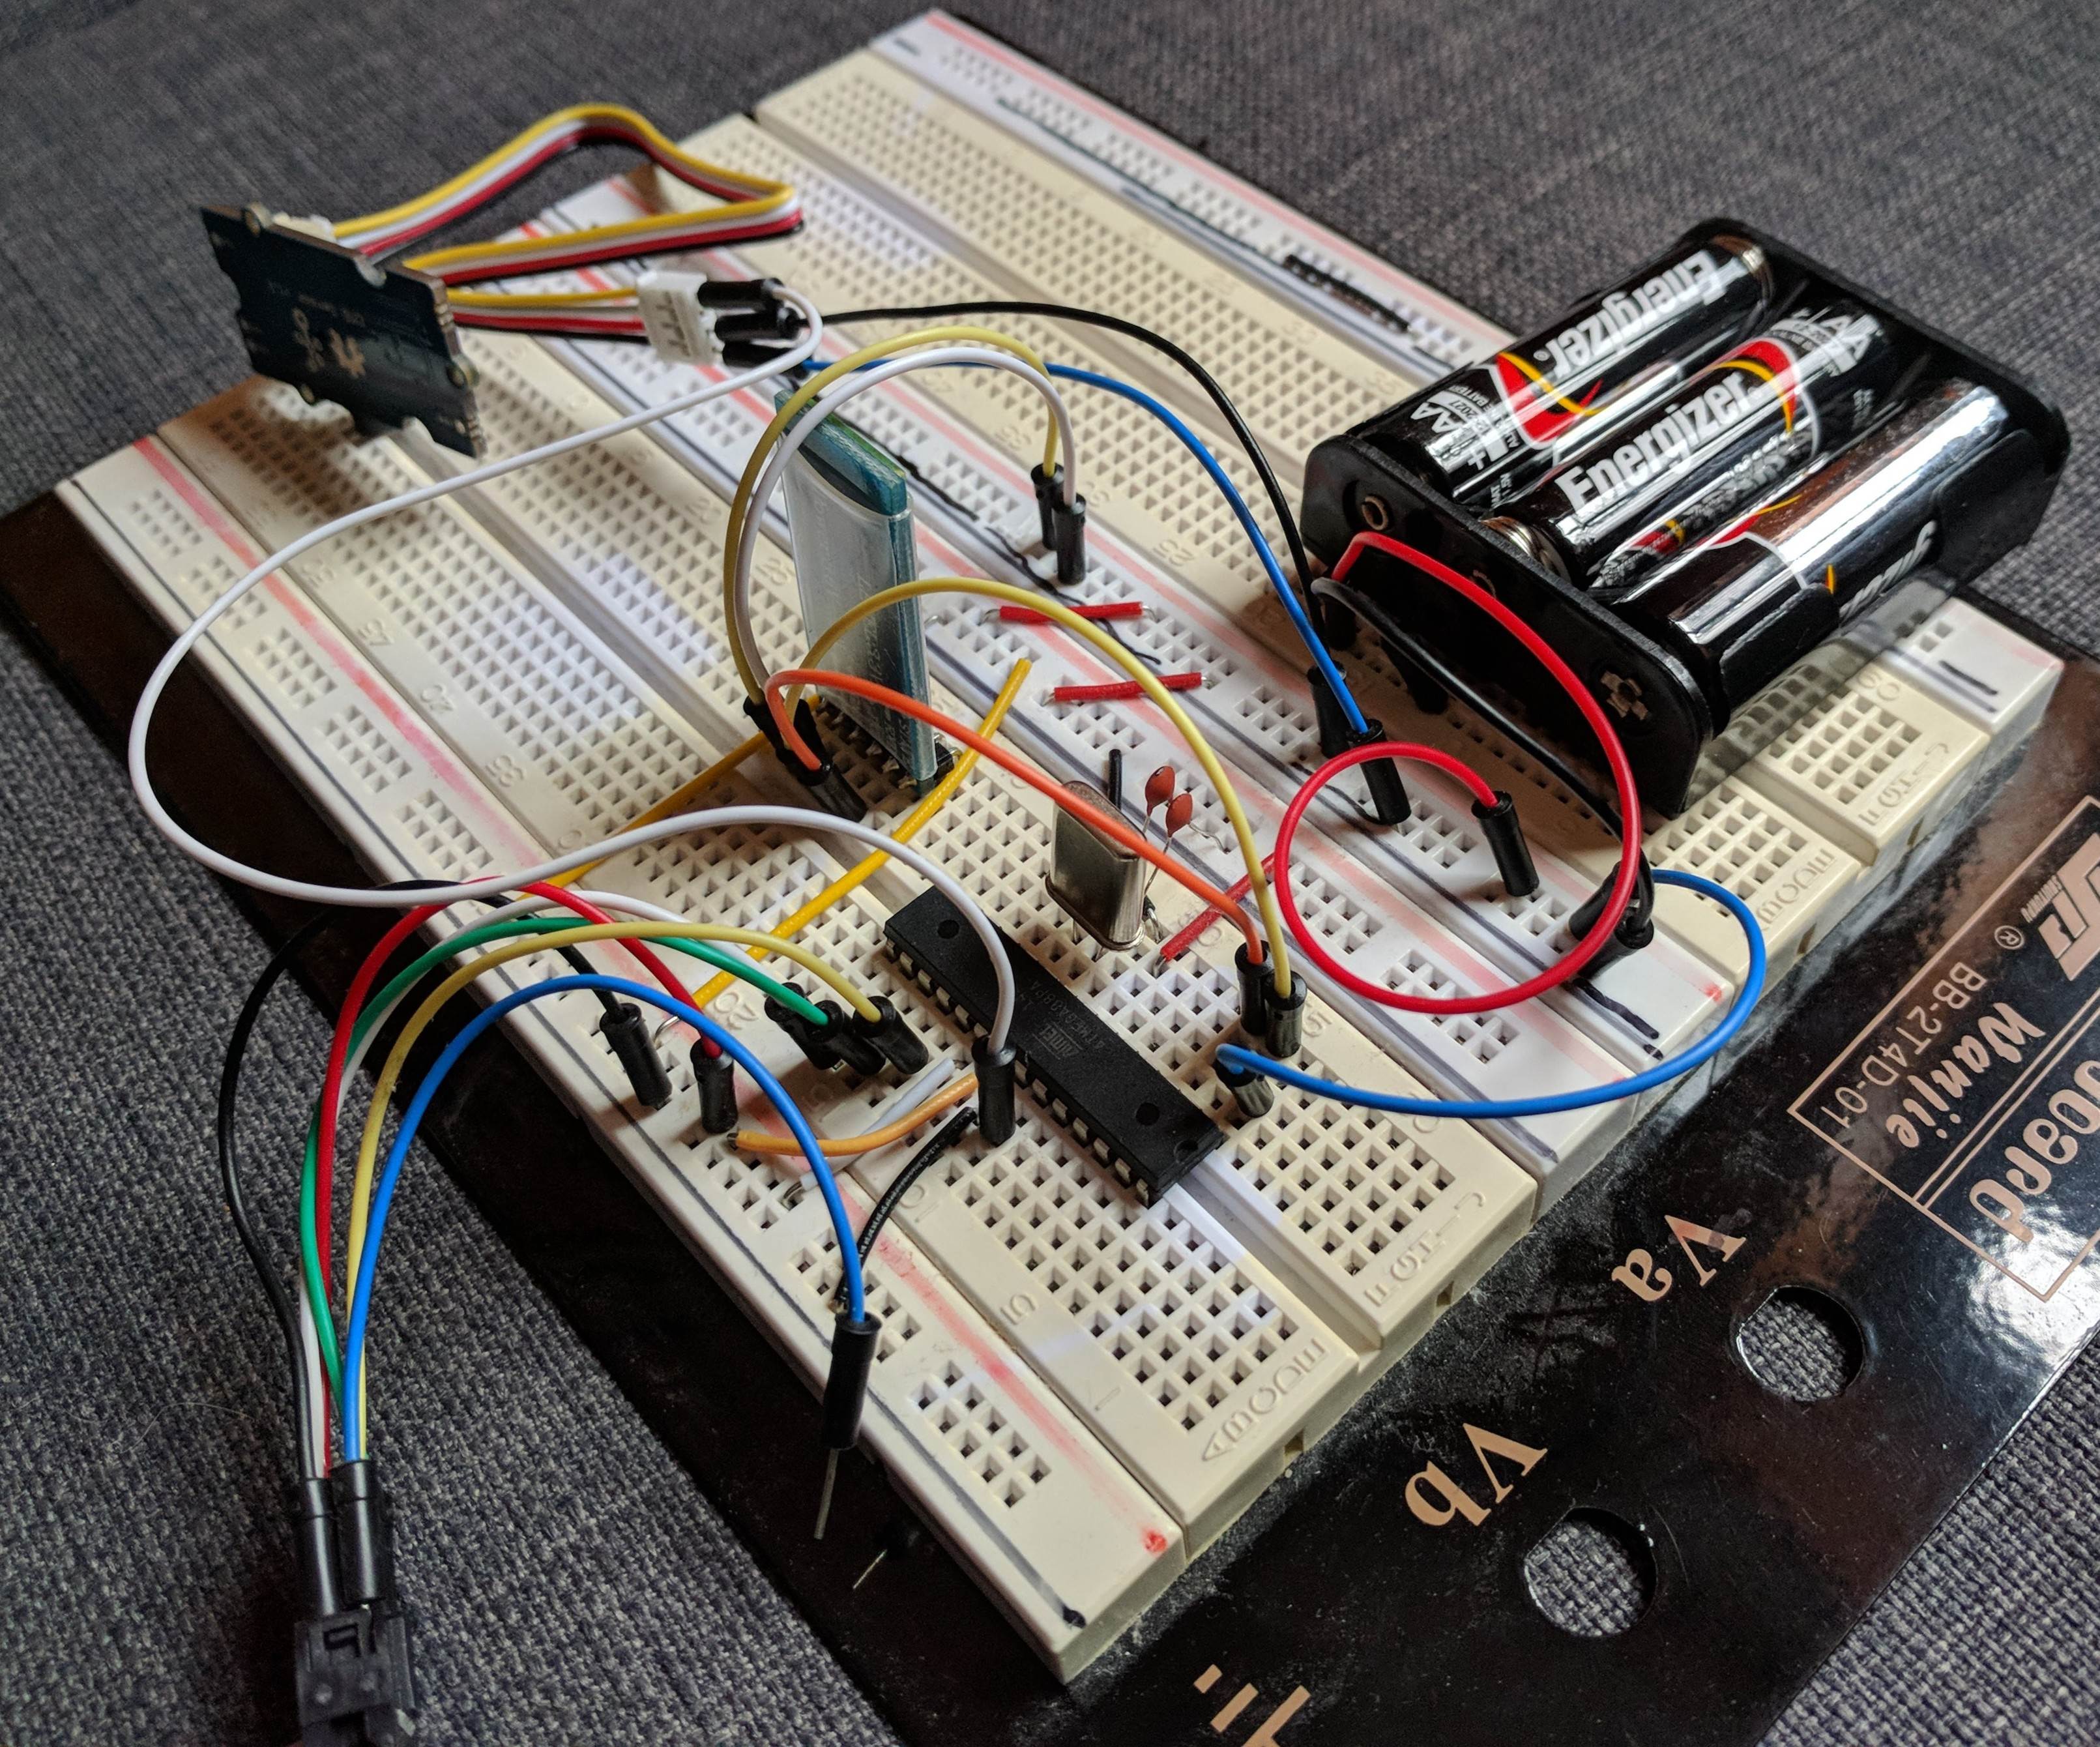
\includegraphics[width=0.8\colwidth]{pics/mikrocontroller}
	  	\caption{aufgebaute Schaltung auf einem Breadboard}
	  	\label{fig:mcspp}
	  \end{figure}
  \end{alertblock}
\end{column}

\separatorcolumn
\begin{column}{\colwidth}  
	
	\begin{alertblock}{Konzept und Aufbau der Begleitapp}
		\begin{itemize}
			\item Durchführung von \textbf{Bewegungsübungen}:
			\begin{itemize}
				\item Messwerte im zeitlichen Verlauf
				\item Vergleich mit früheren Übungen
			\end{itemize}
			\item einfaches \textbf{Minispiel} (durch Bewegungen steuerbar)
			\item verbindendes \textbf{Gamification-System}:
			\begin{itemize}
				\item einfach sichtbar
				\item Experience Points, Badges, Quests
			\end{itemize}
			\item Einteilung in 4 \textbf{Bildschirmseiten} (Activities):
			\begin{itemize}
				\item Startseite (Zusammenfassung der Erfolge, Informationstexte, Verknüpfungen)
				\item Übungsseite (Darstellung der Messwerte, Ansicht der verfügbaren Quests)
				\item Seite für das Minispiel
				\item Einstellungsseite (u.a. für Erinnerungen)
			\end{itemize}
		\end{itemize}
	\end{alertblock}

	\begin{alertblock}{Kommunikation mit dem Gerät}
		\begin{itemize}
			\item Implementierung einer Bluetooth-Verbindung mithilfe des Android-SDK (Software Development Kit)
			\item Verbindung mit dem Gerät in den einzelnen Activities
			\item Einlesen der Bluetooth-Daten mittels einer speziellen Klasse
			\item Ausgleichen von Schwankungen der Messwerte durch eine Warteschlange (Queue)
		\end{itemize}
		\begin{figure}[H]
			\centering
			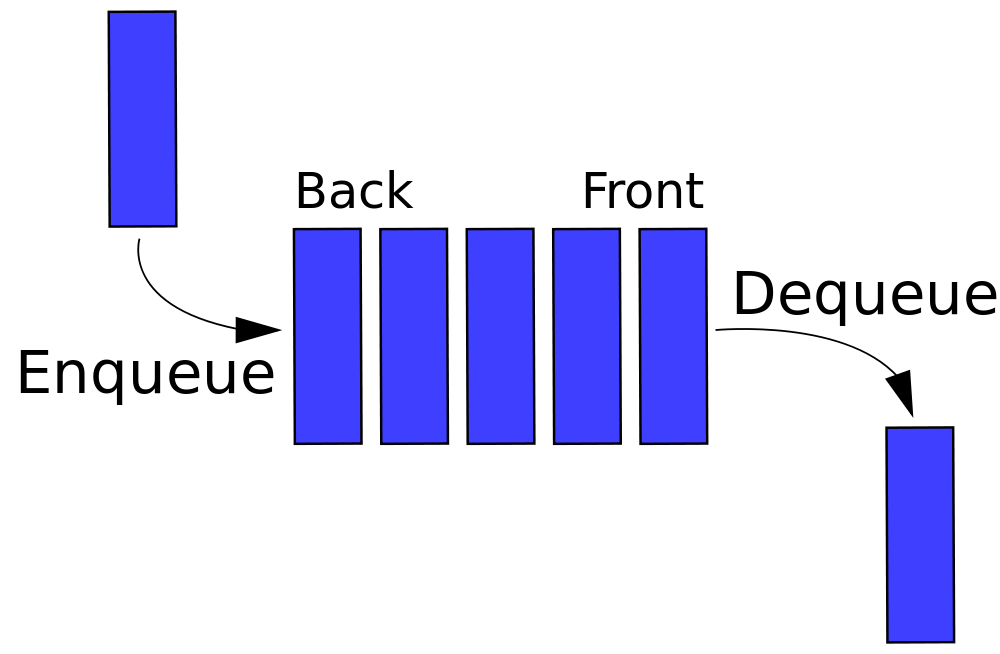
\includegraphics[width=0.5\colwidth]{pics/queue}
			\caption{Funktionsweise einer Queue}
			\label{fig:queue}
		\end{figure}
		\begin{itemize}
			\item Berechnung eines Prozentwerts aus den Messdaten:
			\begin{flalign*}
			& p = 100 * \frac{avg(Q) - U_{min}}{U_{max} - U_{min}}&
			\end{flalign*}
		\end{itemize}
	\end{alertblock}

	\begin{alertblock}{Implementierung der Gamification}
		\begin{itemize}
			\item \textbf{Verteilung der Erfahrungspunkte:}
			\begin{itemize}
				\item abhängig von: Liste der prozentualen Messwerte $L$, Anzahl der Messwerte $d$
				\item Punktzahl $P$ für eine Übung:
				\begin{flalign*}
				& P = \frac{min(L) + avg(L) + max(L)}{3}&
				\end{flalign*}
				\item Punktzahl $P_{S}$ für ein Minispiel:
				\begin{flalign*}
				& P_{S} = P + 2 \cdot d&
				\end{flalign*}
			\end{itemize}
			\item Quests sollen verschiedene Anforderungen zur Fertigstellung voraussetzen
			\item SQL-Datenbank zum Speichern dieser Anforderungen gut geeignet (SQLite)
			\item Aufbau der Datenbanktabelle: Titel, Beschreibung, Symbol, ...
			\item \textbf{mögliche Anforderungen:}
			\begin{enumerate}
				\item bestimmte Anzahl an XP
				\item Messwert einmal während einer Übung erreichen
				\item Messwert über eine bestimmte Zeitspanne halten
			\end{enumerate}
			\item Erfolge werden für den Nutzer sichtbar gemacht (über Dialoge etc.)
		\end{itemize}
	\end{alertblock}

	\begin{alertblock}{Konzept des Minispiels}
		\begin{itemize}
			\item Steuerung eines virtuellen Flugzeuges über eine Gebirgslandschaft mit Bergen unterschiedlicher Höhe
			\item Höhe des Flugzeugs $\sim$ gemessene Muskelaktivität
			\item Ziel: Flugzeug möglichst lange fliegen lassen, ohne gegen Berg zu stoßen
			\item zur Implementierung genutzt: eigenes Android-Obeflächenelement (View)
		\end{itemize}
	\end{alertblock}

\end{column}

\separatorcolumn
\end{columns}
\end{frame}

\end{document}
